\documentclass[a4paper]{article}
\usepackage[utf8]{inputenc}
\usepackage[spanish, es-tabla]{babel}

\usepackage{amsmath}
\usepackage{amsfonts}
\usepackage{amssymb}

\usepackage{float}
\usepackage{graphicx}
\usepackage{subcaption}
\captionsetup{compatibility=false}

\usepackage{multirow}
\setlength{\doublerulesep}{\arrayrulewidth}

\usepackage{array}
\newcolumntype{C}[1]{>{\centering\let\newline\\\arraybackslash\hspace{0pt}}m{#1}}

\usepackage[american]{circuitikz}



\usepackage{fancyhdr}

\usepackage{units} 

\pagestyle{fancy}
\fancyhf{}
\lhead{22.01 TC}
\rhead{Mechoulam, Lambertucci, Rodriguez, Londero, Galdeman}
\rfoot{Página \thepage}
\begin{document}

\tableofcontents
\break
\section{auxiliar}

\subsection{Introducción Teórica}

\subsubsection{Filtros Activos con GIC}

Los inductores suelen ser los componentes electrónicos menos ideales a la hora de querer realizar un filtro. Esto se debe a varias razones: su tamaño en frecuencias bajas y por ende su peso, su resistencia interna grande en comparación a los capacitores, su dificultad a la hora del armado y más. Con el surgimiento del concepto de la realimentación en los circuitos electrónicos, se pudo mediante el uso de amplificadores operacionales, obtener cualquier tipo de respuesta en los filtros. Además, como los operacionales son dispositivos activos, estos pueden proveer al circuito la energía que es disipada por los resistores y aún más por medio de la alimentación que estos dispositivos requieren.

Sin embargo, varias limitaciones surgen por el uso de operacionales. La más importante suele ser la dependencia de la ganancia a lazo abierto con la frecuencia y su inconveniente respuesta a altas frecuencias. Esto suele ocasionar que los filtros activos tengan un rango de correcta operación por debajo de hasta los $100Mhz$. Afortunadamente cuanto mayor la frecuencia menores son las dificultades presentadas por el uso de inductores y esto hace que para este rango de frecuencias el inductor vuelva a ser una buena opción a la hora de implementar filtros.

Varias implementaciones de filtros activos han sido utilizadas históricamente, siendo una de estas el método de la síntesis directa. Este método se basa en utilizar distintos convertidores de impedancia como giradores o GICs. En este informe nos centraremos, entre otras cosas, al análisis e implementación de filtros utilizando el método de síntesis directa, comenzando con una breve explicación del funcionamiento de un GIC.

\subsubsection{Convertidor Generalizado de Impedancia o GIC}
Los convertidores generalizados de impedancia o GICs son circuitos activos diseñados para simular impedancias que cambian con la frecuencia. Se puede observar en la Figura (\ref{fig:gic}) una implementación de un GIC.

\begin{figure} [H]
	\centering
	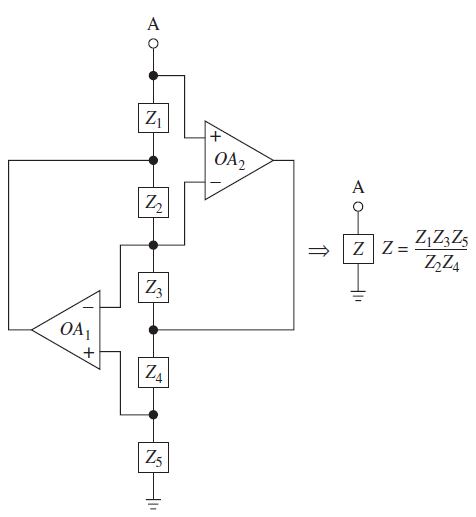
\includegraphics[width=0.6\textwidth]{Imagenes/gic.PNG}
	\caption{Convertidor generalizado de impedancia puesto a tierra[1].}
	\label{fig:gic}
\end{figure}

Estos circuitos están compuestos solamente por resistores, capacitores y amplificadores operacionales, por lo que sobresalen en su uso como emuladores de inductores o capacitores de gran capacidad.

\begin{figure}[H]
	\centering
	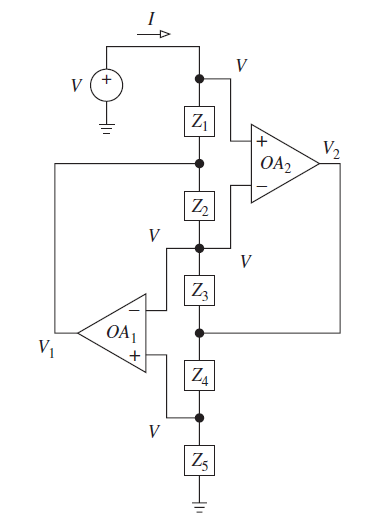
\includegraphics[width=0.5\textwidth]{Imagenes/gic_zin.PNG}
	\caption{Obtención de la impedancia de entrada del convertidor generalizado de impedancia puesto a tierra[2].}
	\label{fig:gic}
\end{figure}

Para obtener la impedancia de entrada del GIC basta solamente calcular la corriente de entrada y utilizar la ley de nodos de Kirchhoff en los nodos de potencial V.

\begin{equation}
\frac{V-V_1}{Z_1}=I
\label{gic_zin_1}
\end{equation}

\begin{equation}
\frac{V_1-V}{Z_2} = \frac{V-V_2}{Z_3}
\label{gic_zin_2}
\end{equation}

\begin{equation}
\frac{V_2-V}{Z_4} = \frac{V}{Z_5}
\label{gic_zin_3}
\end{equation}

Utilizando (\ref{gic_zin_1}), (\ref{gic_zin_2}) y (\ref{gic_zin_3}) se llega finalmente a

\begin{equation}
Z_{in} = \frac{Z_1 Z_3 Z_5}{Z_2 Z_4}
\label{grounded_gic_zin}
\end{equation}

Esto demuestra que un GIC se puede utilizar para emular la impedancia que se desee, eligiendo convenientemente las impedancias $Z_1, \ Z_2, \ Z_3, \ Z_4 \ y \ Z_5$ dentro de las limitaciones que este posee.

\begin{figure}[H]
	\centering
	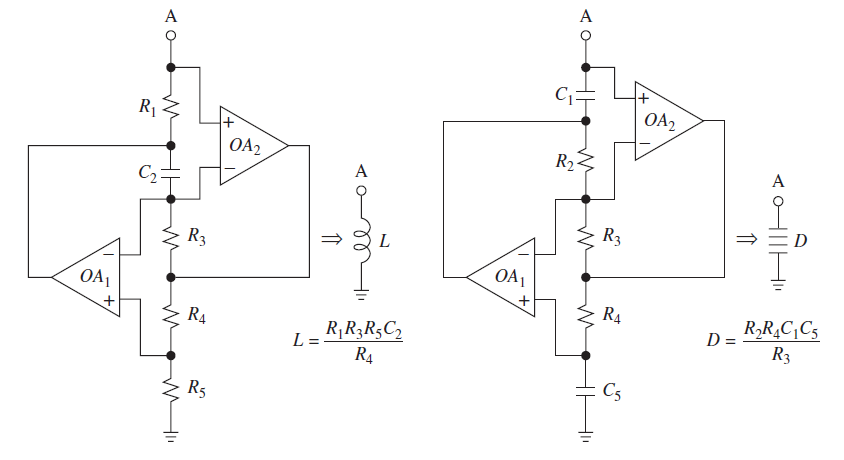
\includegraphics[width=1\textwidth]{Imagenes/gic_ind_fndr.PNG}
	\caption{Utilización de GICs para emular una inductancia a la izquierda y realizar un FNDR o elemento D a la derecha[3].}
	\label{fig:gic_ind_fndr}
\end{figure}

Como se puede observar en la Figura (\ref{fig:gic_ind_fndr}), dos implementaciones muy utilizadas de los GICs puestos a tierra son la de un inductor puesto a tierra o un FNDR. Sin embargo, estas implementaciones poseen varias limitaciones a la hora de realizar el diseño de un filtro ya que por la naturaleza interna de los amplificadores operacionales, se debe tener en cuenta que debe haber un camino para la continua que pueda ser utilizada para polarizar correctamente los transistores en el interior de los operacionales. En el siguiente circuito se analizará e implementará un filtro activo con un GIC no puestoa tierra.


\subsection{Análisis del Circuito}
\subsubsection{Análisis de la Función Transferencia}

\subsubsection{Análisis de Polos y Ceros}
\subsubsection{Análisis de Impedancias de Entrada y Salida}
\subsubsection{Análisis Funcional de los Componentes}
\subsubsection{Análisis de Sensibilidades}
\subsubsection{Elección de Componentes y sus Tecnologías}

\subsection{Simulación del Circuito}
\subsubsection{Simulación de la Transferencia}
\subsubsection{Simulación de la Impedancia de Entrada y Salida}
\subsubsection{Simulación de las Sensibilidades}
\subsubsection{Conclusiones Adquiridas}

\subsection{Prototipo del Circuito}
\subsubsection{Mediciones del Prototipo}
\subsubsection{Conclusiones Adquiridas}

\subsection{Implementación del Circuito}
\subsubsection{Mediciones del Circuito y Análisis de Error}
\subsubsection{Limitaciones del Circuito}

\subsection{Conclusiones}

\subsection{Bibliografía Utilizada}
[1]F. Sergio, Design with operational amplifiers and analog integrated circuits, 4th ed. New York [etc.]: McGraw-Hill, 1988, p. 185.
[2]F. Sergio, Design with operational amplifiers and analog integrated circuits, 4th ed. New York [etc.]: McGraw-Hill, 1988, p. 186.
[3]F. Sergio, Design with operational amplifiers and analog integrated circuits, 4th ed. New York [etc.]: McGraw-Hill, 1988, p. 187.

\begin{equation}
\hspace{-4cm}
\frac{vi \left(- C_{2} C_{6}^{2} C_{7} R_{1} R_{3} R_{4} R_{6}^{2} R_{7}^{2} S^{4} - C_{2} C_{6}^{2} R_{1} R_{3} R_{4} R_{6}^{2} R_{7} S^{3} + C_{2} C_{6} C_{7}^{2} R_{1} R_{3} R_{6}^{2} R_{7}^{2} R_{8} S^{4} - 2 C_{2} C_{6} C_{7} R_{1} R_{3} R_{4} R_{6} R_{7}^{2} S^{3} + 2 C_{2} C_{6} C_{7} R_{1} R_{3} R_{6}^{2} R_{7} R_{8} S^{3} - C_{2} C_{6} R_{1} R_{3} R_{4} R_{6}^{2} R_{7}^{2} S^{2} - 2 C_{2} C_{6} R_{1} R_{3} R_{4} R_{6} R_{7} S^{2} + C_{2} C_{6} R_{1} R_{3} R_{6}^{2} R_{8} S^{2} + C_{2} C_{7}^{2} R_{1} R_{3} R_{6} R_{7}^{2} R_{8} S^{3} - C_{2} C_{7} R_{1} R_{3} R_{4} R_{7}^{2} S^{2} + C_{2} C_{7} R_{1} R_{3} R_{6}^{2} R_{7}^{2} R_{8} S^{2} + 2 C_{2} C_{7} R_{1} R_{3} R_{6} R_{7} R_{8} S^{2} - C_{2} R_{1} R_{3} R_{4} R_{6} R_{7}^{2} S - C_{2} R_{1} R_{3} R_{4} R_{7} S + C_{2} R_{1} R_{3} R_{6}^{2} R_{7} R_{8} S + C_{2} R_{1} R_{3} R_{6} R_{8} S + C_{6}^{2} R_{4} R_{6}^{2} R_{7}^{2} S^{2} + C_{6} C_{7} R_{4} R_{6}^{2} R_{7}^{2} S^{2} + C_{6} R_{4} R_{6}^{2} R_{7} S + 2 C_{6} R_{4} R_{6} R_{7}^{2} S + C_{7} R_{4} R_{6} R_{7}^{2} S + R_{4} R_{6} R_{7} + R_{4} R_{7}^{2}\right)}{C_{2} C_{6}^{2} C_{7} R_{1} R_{3} R_{6}^{2} R_{7}^{2} R_{8} S^{4} + C_{2} C_{6}^{2} R_{1} R_{3} R_{6}^{2} R_{7} R_{8} S^{3} + C_{2} C_{6} C_{7}^{2} R_{1} R_{3} R_{6}^{2} R_{7}^{2} R_{8} S^{4} + 2 C_{2} C_{6} C_{7} R_{1} R_{3} R_{6}^{2} R_{7} R_{8} S^{3} + 2 C_{2} C_{6} C_{7} R_{1} R_{3} R_{6} R_{7}^{2} R_{8} S^{3} + C_{2} C_{6} R_{1} R_{3} R_{6}^{2} R_{7}^{2} R_{8} S^{2} + C_{2} C_{6} R_{1} R_{3} R_{6}^{2} R_{8} S^{2} + 2 C_{2} C_{6} R_{1} R_{3} R_{6} R_{7} R_{8} S^{2} + C_{2} C_{7}^{2} R_{1} R_{3} R_{6} R_{7}^{2} R_{8} S^{3} + C_{2} C_{7} R_{1} R_{3} R_{6}^{2} R_{7}^{2} R_{8} S^{2} + 2 C_{2} C_{7} R_{1} R_{3} R_{6} R_{7} R_{8} S^{2} + C_{2} C_{7} R_{1} R_{3} R_{7}^{2} R_{8} S^{2} + C_{2} R_{1} R_{3} R_{6}^{2} R_{7} R_{8} S + C_{2} R_{1} R_{3} R_{6} R_{7}^{2} R_{8} S + C_{2} R_{1} R_{3} R_{6} R_{8} S + C_{2} R_{1} R_{3} R_{7} R_{8} S + C_{6}^{2} R_{4} R_{6}^{2} R_{7}^{2} S^{2} + C_{6} C_{7} R_{4} R_{6}^{2} R_{7}^{2} S^{2} + C_{6} R_{4} R_{6}^{2} R_{7} S + 2 C_{6} R_{4} R_{6} R_{7}^{2} S + C_{7} R_{4} R_{6} R_{7}^{2} S + R_{4} R_{6} R_{7} + R_{4} R_{7}^{2}}
\end{equation}


\end{document}